\documentclass[14pt, aspectratio=169, handout]{beamer}
\usetheme{Copenhagen}
\usecolortheme{seahorse}
\setbeamertemplate{navigation symbols}{}
\setbeamertemplate{headline}{}

%\usepackage{pgfpages}
%\pgfpagesuselayout{4 on 1}[a4paper, border shrink=5mm]

\usepackage{graphicx} % Required for inserting images
\usepackage{multicol}
%\usepackage{enumitem}
\usepackage{amsfonts}
\usepackage{amsmath}
\usepackage{xcolor}
\definecolor{myblue}{RGB}{0, 0, 255} 
\definecolor{mygreen}{RGB}{0, 180, 80}
\definecolor{myred}{RGB}{153, 0, 0}
\definecolor{myorange}{RGB}{255, 153, 51}
\definecolor{mypurple}{RGB}{102, 0, 204}
\usepackage{tikz}

%--- commands for transform arrows----------------
\newcommand{\transform}[2]{%
    \begin{tikzpicture}
        % Open circle
        \draw[thick] (0,0) circle (0.1);
        % Line with number above and adjustable length
        \draw[thick] (0.1,0) -- (#2,0) node[midway, above] {#1};
        % Filled circle
        \filldraw[thick] (#2,0) circle (0.1);
    \end{tikzpicture}%
}
\newcommand{\invtransform}[2]{%
    \begin{tikzpicture}
        % filled circle
        \filldraw[thick] (0,0) circle (0.1);
        % Line with number above and adjustable length
        \draw[thick] (0.1,0) -- (#2 -0.1,0) node[midway, above] {#1};
        % open circle
        \draw[thick] (#2,0) circle (0.1);
    \end{tikzpicture}%
}
\newcommand{\verticaltransform}[4]{%
    \begin{tikzpicture}
        % Open circle at the bottom with text below
        \filldraw[thick] (0,0) circle (0.1) node[below=3pt] {$#4$};
        % Vertical line with number on the left
        \draw[thick] (0,0.1) -- (0,#2 -0.1) node[midway, left] {#1};
        % Filled circle at the top with text above
        \draw[thick] (0,#2) circle (0.1) node[above=3pt] {$#3$};
    \end{tikzpicture}%
}
\newcommand{\verticalinvtransform}[4]{%
    \begin{tikzpicture}
        % Open circle at the bottom with text below
        \draw[thick] (0,0) circle (0.1) node[below=3pt] {$#4$};
        % Vertical line with number on the left
        \draw[thick] (0,0.1) -- (0,#2) node[midway, left] {#1};
        % Filled circle at the top with text above
        \filldraw[thick] (0,#2) circle (0.1) node[above=3pt] {$#3$};
    \end{tikzpicture}%
}

\definecolor{darkblue}{RGB}{0, 0, 139}
\definecolor{lightblue}{RGB}{173, 216, 230}

\title{SST1 Übungsstunde 12}
\author{Matteo Dietz}
\date{December 2024}

\begin{document}

\maketitle

\begin{frame}{Themenüberblick}
    \begin{itemize}
        \item \textbf{Repetition: Diskrete Fouriertransformation (DFT)}
        \item[] Visualisierung, Matrixdarstellung, Zyklische Faltung
        \item[] Diskrete Filter, Überabtastung, Unterabtastung
        \item[] 
        \item \textbf{Fast Fourier Transform (FFT)}
        \item[] Cooley-Tukey FFT
        \item[] 
        \item \textbf{Tipps für die Prüfung}
    \end{itemize}
\end{frame}

\begin{frame}{Aufgaben für diese Woche}
    \begin{itemize}
        \item[] \textbf{123}, \textbf{124}, \textbf{125}, \textbf{126}, \textbf{127}, \textbf{128}, \textbf{129}, \textbf{130}, \textbf{131}
        \item[] 
        \item[] Die \textbf{fettgedruckten} Übungen empfehle ich, weil sie wesentlich zu eurem Verständnis der Theorie beitragen und/oder sehr prüfungsrelevant sind.
        \item[] 
        \item[] Die DFT ist \textcolor{myred}{sehr wichtig}! Es kommt immer eine ganze Aufgabe dazu an der Prüfung. (25 / 100 Punkte)
    \end{itemize}
\end{frame}

\begin{frame}{Diskrete Fouriertransformation (DFT)}
    \fcolorbox{darkblue}{lightblue}{%
    \parbox{\dimexpr\linewidth-2\fboxsep-2\fboxrule\relax}{
    \vspace*{0.15cm}
    \begin{itemize}
        \item[] $(\textbf{DFT}) \hspace{40pt} \hat{x}[k] = \displaystyle\sum_{n=0}^{N-1} x[n]\omega_N^{kn} \hspace{50pt} \hat{x}[k+N] = \hat{x}[k]$
        \item[] $(\textbf{IDFT}) \hspace{36pt} x[n]=\displaystyle\frac{1}{N}\displaystyle\sum_{k=0}^{N-1} \hat{x}[k] \omega_N^{-kn} \hspace{42pt} x[n+N] = x[n]$
        \item[] wobei $\hspace{48pt} \omega_N = e^{-\frac{2 \pi i}{N}}$
    \end{itemize}
}}%
\end{frame}

\begin{frame}{DFT: Visualisierung}
    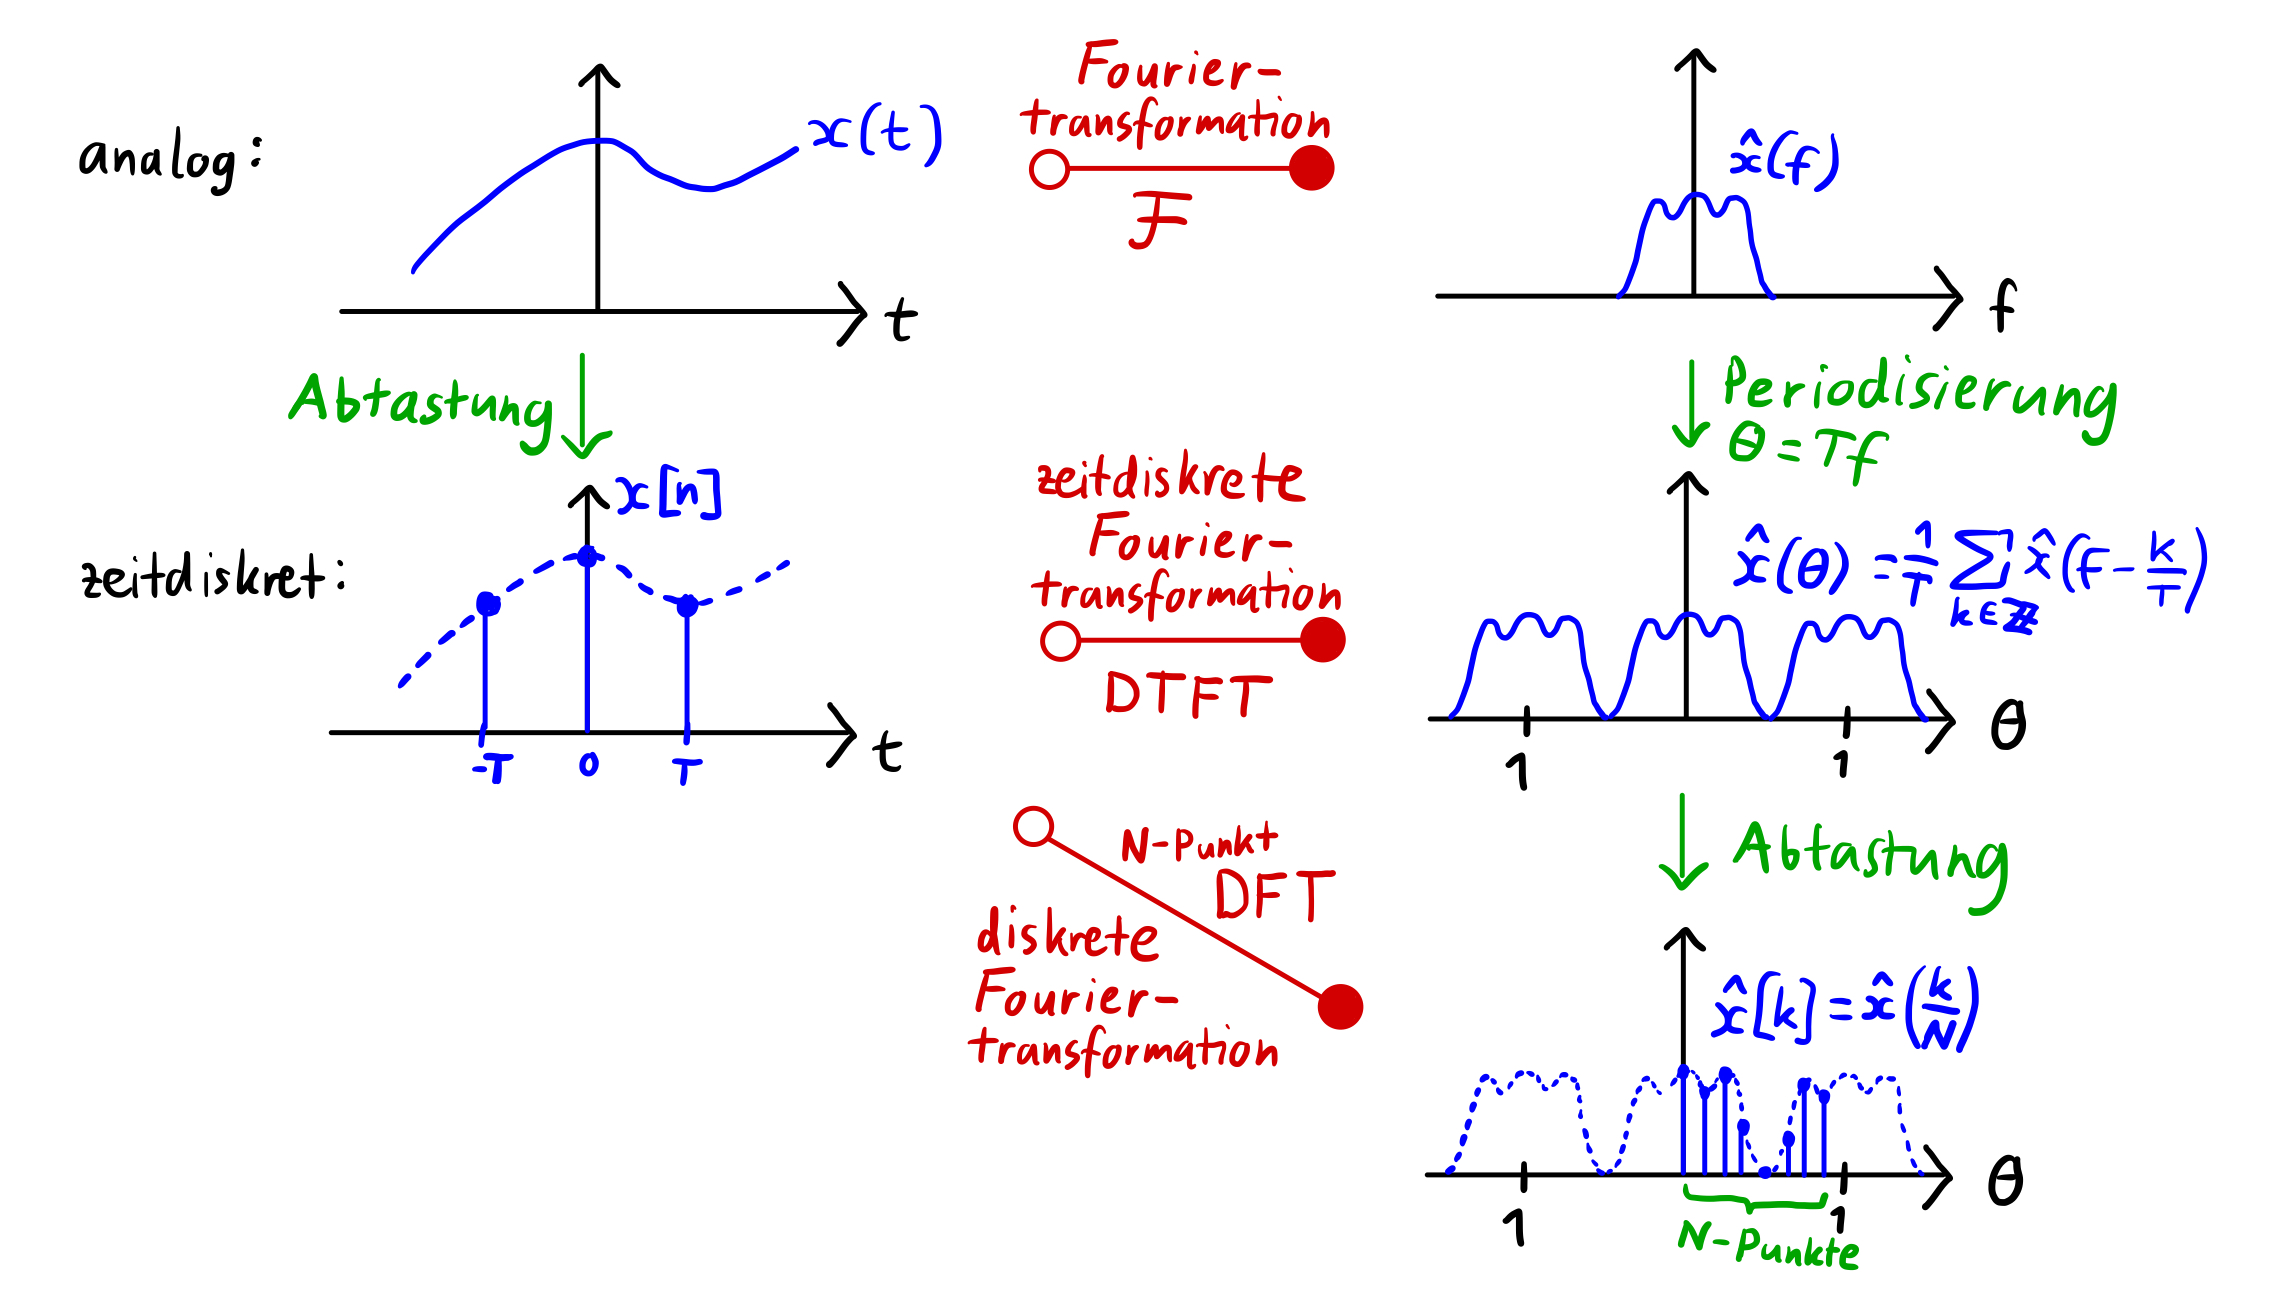
\includegraphics[width=0.95\linewidth]{figures/DFT_visuals.jpeg}
\end{frame}

\begin{frame}{DFT: Matrixdarstellung}
    Wir haben $\hat{x}[k] = \displaystyle\sum_{n=0}^{N-1} x[n]\omega_N^{kn}, \hspace{20pt} k \in \{ 0, \; 1, \; \dots, \; N-1 \}$ Somit:

$$\underbrace{\begin{bmatrix}
    \hat{x}[0] \\
    \hat{x}[1] \\
    \hat{x}[2] \\
    \vdots \\
    \hat{x}[N-1]
\end{bmatrix}}_{=: \hat{\mathbf{x}}} = \underbrace{\begin{bmatrix}
    1 & 1 & 1 & \cdots & 1 \\
    1 & \omega_N & \omega_N^2 & \cdots & \omega_N^{N-1} \\
    1 & \omega_N^2 & \omega_N^4 & \cdots & \omega_N^{2(N-1)} \\
    \vdots & \vdots & \vdots & \ddots & \vdots \\
    1 & \omega_N^{N-1} & \omega_N^{2(N-1)} & \cdots & \omega_N^{(N-1)^2}
\end{bmatrix}}_{\text{DFT-Matrix } F_N} \underbrace{\begin{bmatrix}
    x[0] \\
    x[1] \\
    x[2] \\
    \vdots \\
    x[N-1]
\end{bmatrix}}_{\mathbf{x}}$$

\end{frame}

\begin{frame}{DFT: Matrixdarstellung}
    
\fcolorbox{darkblue}{lightblue}{%
    \parbox{\dimexpr\linewidth-2\fboxsep-2\fboxrule\relax}{
        Somit erhalten wir: \\
        \noindent
        \begin{minipage}[t]{0.45\textwidth}
            \vspace*{0.1cm}
            \begin{itemize}
                \item[] \textbf{DFT}
                \item[] $\hat{\mathbf{x}} = F_N \mathbf{x}$
            \end{itemize}
            \vspace*{0.1cm}
        \end{minipage}%
        \hfill%
        \begin{minipage}[t]{0.45\textwidth}
            \vspace*{0.1cm}
            \begin{itemize}
                \item[] \textbf{IDFT}
                \item[] $\mathbf{x} = \frac{1}{N}F_N^H \hat{\mathbf{x}}$
            \end{itemize}
            \vspace*{0.1cm}
        \end{minipage}
    }%
}

\begin{itemize}
    \item[] 
    \item[] 
    \item[] Die Spalten von $F_N$ sind orthogonal aufeinander: $\langle \mathbf{f}_r, \; \mathbf{f}_s \rangle = \delta_{r,s}$
    \item[] 
    \item[] Es gilt $F_N F_N^H = N I_N$
\end{itemize}
\end{frame}

\begin{frame}{Formelsammlung: DFT Eigenschaften}
    \begin{center}
        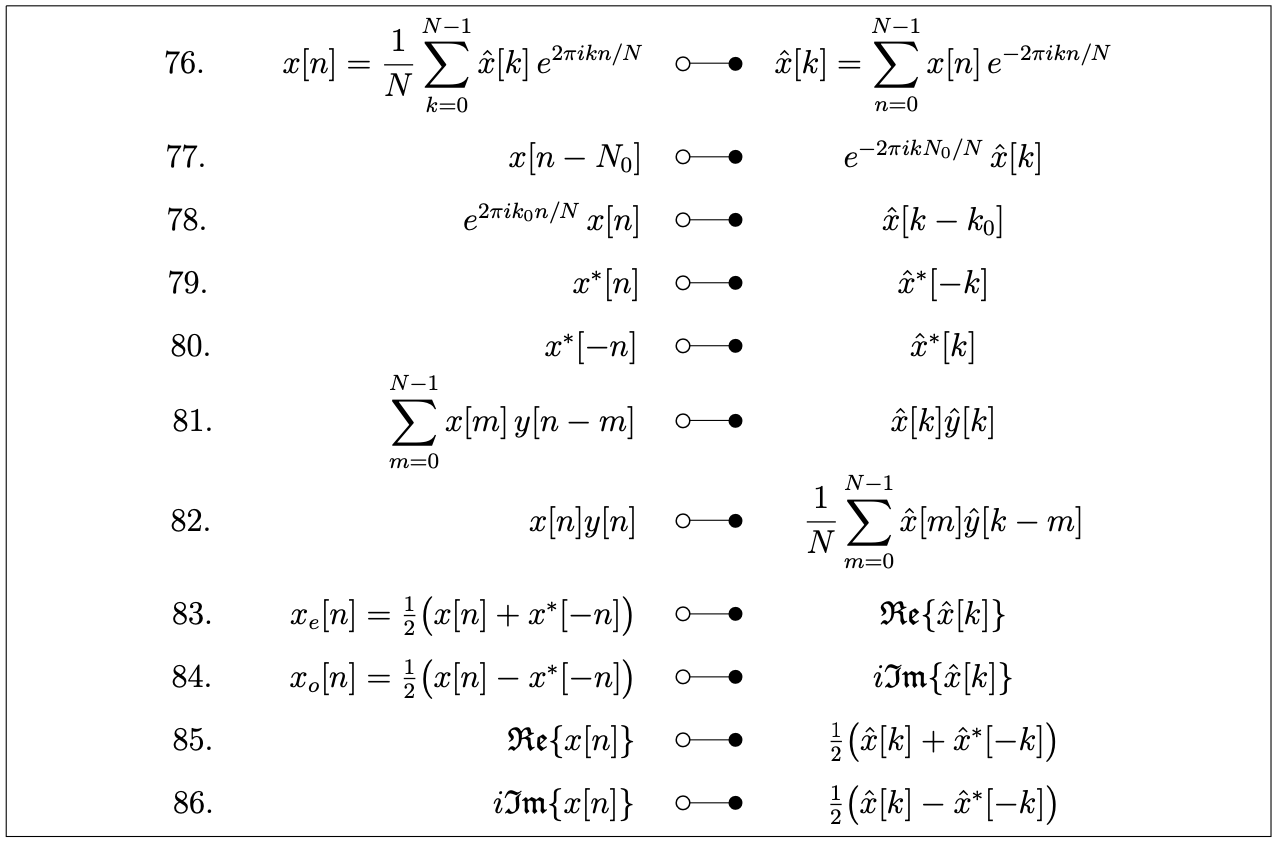
\includegraphics[width=0.75\linewidth]{figures/DFT_Eigenschaften.png}
    \end{center}
\end{frame}

\begin{frame}{Formelsammlung: DFT Transformationspaare}
    \begin{center}
        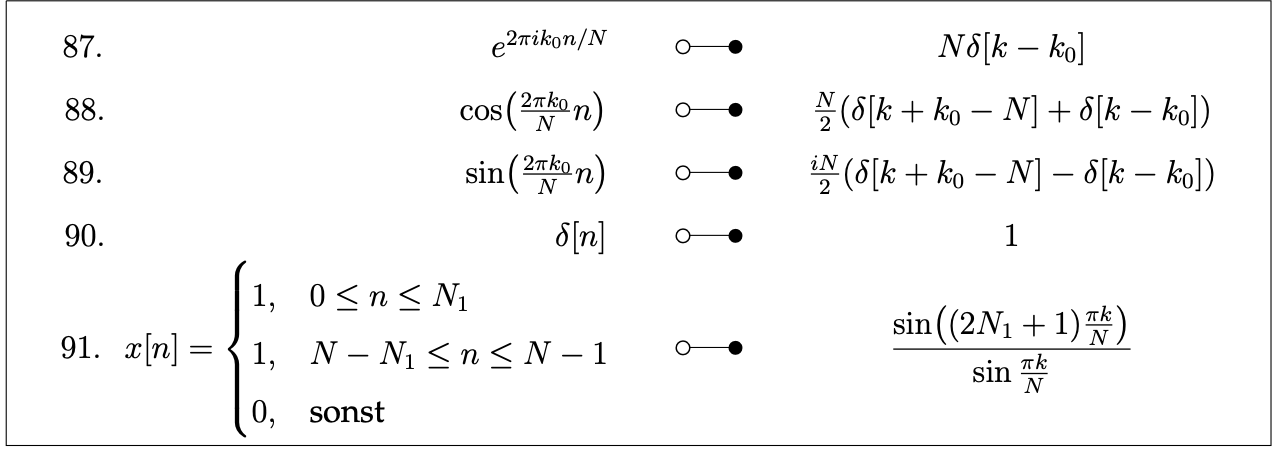
\includegraphics[width=\linewidth]{figures/DFT_Paare.png}
    \end{center}
\end{frame}

\begin{frame}{Zyklische Faltung}
    \fcolorbox{darkblue}{lightblue}{%
    \parbox{\dimexpr\linewidth-2\fboxsep-2\fboxrule\relax}{
    \vspace*{0.15cm}
    $$\vspace*{-0.5cm} x_3[l] = \sum_{n=0}^{N-1} x_1[n]x_2[l-n] = \sum_{n=0}^{N-1} x_1[l-n] x_2[n]$$
    $$\vspace*{-0.5cm}\verticaltransform{\text{DFT}}{1}{}{} \hspace{58pt}$$
    $$\hat{x}_3[k] = \hat{x}_1[k] \cdot \hat{x}_2[k]$$
}}%

\vspace*{0.5cm}
\textbf{Elementweise Multiplikation im Frequenzbereich entspricht einer zyklischen Faltung im Zeitbereich}
\end{frame}

\begin{frame}{Zyklische Faltung: Matrixdarstellung}

    $$x_3[l] = \sum_{n=0}^{N-1} x_1[n]x_2[l-n] = \sum_{n=0}^{N-1} x_1[l-n] x_2[n]$$

$$\underbrace{\begin{bmatrix}
        x_3[0] \\
        x_3[1] \\
        \vdots \\
        x_3[N-1]
    \end{bmatrix}}_{\mathbf{x}_3} 
    = \underbrace{\begin{bmatrix}
        x_2[0] & x_2[N-1] & \cdots & x_2[1] \\
        x_2[1] & x_2[0] & \cdots & x_2[2] \\
        \vdots & \vdots & \ddots & \vdots \\
        x_2[N-1] & x_2[N-2] & \cdots & x_2[0]
    \end{bmatrix}}_{\mathbf{X}_2} \underbrace{\begin{bmatrix}
        x_1[0] \\
        x_1[1] \\
        \vdots \\
        x_1[N-1]
    \end{bmatrix}}_{\mathbf{x}_1}$$
\end{frame}

\begin{frame}{Zyklische Faltung: Matrixdarstellung}
  $$ \mathbf{X}_2 = \frac{1}{N} \mathbf{F}_N^H  \begin{bmatrix}
        \hat{x}_2[0] & & \mathbf{0} \\
        & \ddots & \\
        \mathbf{0} & & \hat{x}_2[N-1]
    \end{bmatrix}  \mathbf{F}_N $$

    \begin{enumerate}
        \item[]
        \item \textbf{Die zyklische Faltung wird durch die DFT diagonalisiert}.
        \item[] 
        \item Eigenvektoren einer zirkulanten Matrix $=$ Spalten der normalisierten DFT-Matrix $\frac{1}{\sqrt{N}}\mathbf{F}_N^H$
    \end{enumerate}
\end{frame}

\begin{frame}{Diskrete Filter}
    
\end{frame}

\begin{frame}{Diskrete Filter: Matrixdarstellung}
    
\end{frame}

\begin{frame}{DFT: Kritische Abtastung}
    
\end{frame}

\begin{frame}{DFT: Überabtastung}
    
\end{frame}

\begin{frame}{DFT: Unterabtastung}
    
\end{frame}

\begin{frame}{Fast Fourier Transform (FFT)}
    
\end{frame}

\begin{frame}{Fast Fourier Transform (FFT)}
    
\end{frame}

\begin{frame}{FFT: Rekursionsbaum}
    
\end{frame}

\begin{frame}{FFT: Cooley-Tukey Algorithmus}
    
\end{frame}

\begin{frame}{FFT: Cooley-Tukey Algorithmus}
    
\end{frame}

\begin{frame}{Prüfungsaufgabe: Sommer 2021, Aufgabe 3}
    
\end{frame}

\begin{frame}{Prüfungsinformationen}
    \begin{itemize}
        \item Die Prüfung dauert 180 min (3 Stunden).
        \item[] 
        \item Es gibt 4 Aufgaben, die je 25 Punkte geben. (ca. 45 min pro Aufgabe)
        \item[]
        \item Einziges Hilfsmittel ist die Formelsammlung.
    \end{itemize}
\end{frame}

\begin{frame}{Kontur der Prüfung}
    \begin{enumerate}
        \item Analoge Signale und Systeme, Systemeigenschaften
        \item[] 
        \item Abtasttheorem (Mischung analoge und zeitdiskrete Signale)
        \item[] 
        \item Zeitdiskrete Signale (entweder DTFT oder $\mathcal{Z}-$Transformation)
        \item[] 
        \item DFT
    \end{enumerate}
\end{frame}

\begin{frame}{Tipps für die Prüfung}
    \begin{itemize}
        \item 20 alte Prüfungen. Löst möglichst viele davon!
        \item[] 
        \item Die neueren Prüfungen sind relevanter.
        \item[] 
        \item Nur 4 alte Prüfungen enthalten Aufgaben zu der $\mathcal{Z}-$ Transformation. Schaut Aufgaben 114-122 dazu nochmals an!
        \item[] 
        \item Konzepte wie z.B. das Abtasttheorem gut verstehen!
    \end{itemize}
\end{frame}

\begin{frame}{Tipps für die Prüfung}
    \begin{itemize}
        \item Substitutionen in Integralen und Summen müssen sitzen!
        \item[] 
        \item Lösungswege, Achsenbeschriftungen bei Skizzen etc. nicht vergessen!
        \item[] 
        \item Falls ihr Teilaufgaben nicht schafft, könnt ihr, wenn ihr übrige Zeit habt, trotzdem weiterrechnen (z.B. mit Parametern), vielleicht bekommt ihr dafür einige Punkte.
    \end{itemize}
\end{frame}

\end{document}